\documentclass{article}
\usepackage{graphicx}
\usepackage{amsmath}
\usepackage{amsfonts} 
% or 
\usepackage{amssymb}

\usepackage{mathtools}

\usepackage{tikz}
\usepackage{pgfplots}
\usepgfplotslibrary{fillbetween}
\usetikzlibrary{patterns}

\pgfplotsset{compat = newest}
\usepackage{cancel}
\usepackage[margin=1in]{geometry}

\begin{document}

\title{Maths Lessons}
\maketitle

\section{Quadratics}
Quadratics are second degree polynomials. They usually contain an $x^2$ and can be written
in the form $ax^2 + bx + c$.
\\
The 4 main methods of solving quadratics are as follows:
\begin{itemize}
	\item Factorise
	\item Quadratic Formula
	\item Complete the Square
	\item Graphically
\end{itemize}

\subsection{Quadratic Formula}
The quadratic formula is used to find the solution to arbitrary quadratics in the form $ax^2 + bx + c$. It is as follows:

\begin{equation}
	\frac{-b \pm \sqrt{b^2 - 4ac}}{2a}
\end{equation}

\subsubsection{Deriving the Quadratic fromula}
The quadratic fromula is derived from completing the square. Completing the square is the first step
\begin{gather*}
	ax^2 + bx + c = 0\\
	a \left (x + \frac{b}{2a} \right )^2 - a\left (\frac{b}{2a} \right )^2 + c = 0 \\
	a \left (x + \frac{b}{2a} \right )^2 - \frac{b^2}{4a} + c = 0 \\
	a \left (x + \frac{b}{2a} \right )^2 = \frac{b^2}{4a} - c \\
	\left (x + \frac{b}{2a} \right )^2 = \frac{b^2}{4a^2} - \frac{c}{a} \\
	\left (x + \frac{b}{2a} \right )^2 = \frac{b^2 - 4ac}{4a^2} \\
	x + \frac{b}{2a} = \pm \sqrt{\frac{b^2 - 4ac}{4a^2}} \\
	x + \frac{b}{2a} = \frac{\pm \sqrt{b^2 - 4ac}}{2a} \\
	x = \frac{-b \pm \sqrt{b^2 - 4ac}}{2a} \\
\end{gather*}

\subsubsection{Discriminant}
The discriminant is part of the quadratic formula that can tell us various properties of the parabola.
The discriminant is as follows:
\begin{equation}
	D = b^2 - 4ac
\end{equation}
When the discriminant is positive we have two solutions:
\begin{equation}
	D > 0
\end{equation}
When the discriminant is equal to $0$ we have one solution:
\begin{equation}
	D = 0
\end{equation}
When the discriminant is negative we have no real solutions:
\begin{equation}
	D < 0
\end{equation}
Instead we have complex solutions in the form $ai$ where $i = \sqrt{-1}$.

\subsection{Solving Hidden Quadratics by Substitution}

Given a quadratic such as $2^{2n} + 2 \left ( 4^{n} \right ) + 1$ we can solve by putting in the form
$ax^2 + bx + c$.

\begin{gather}
	2^{2n} + 2 \left ( 2^{n} \right ) + 1 = 0 \\
	\left ( 2^n \right ) ^2 + 2 \left (2^n \right ) + 1 = 0 \\
\end{gather}

\section{Trig}

\begin{equation}
	\sec \theta \equiv \frac{1}{\sin \theta}
\end{equation}


\begin{equation}
	\mathrm{cosec} \theta \equiv \frac{1}{\cos \theta}
\end{equation}

\begin{equation}
	\cot \theta \equiv \frac{1}{\tan \theta}
\end{equation}

\begin{equation}
	\sin^2 \theta  + \cos^2 \theta \equiv 1
\end{equation}

\begin{equation}
	\tan^2 \theta + 1 \equiv \sec^2 \theta
\end{equation}

\begin{equation}
	1 + \cot^2 \theta \equiv \mathrm{cosec}^2 x
\end{equation}

\section{Calculus}

Differentiation, finding a function for the gradient.

\begin{gather*}
	f(x)\\
	m = \frac{y - y_1}{x - x_1}\\
	h = x - x_1 \\
	\text{We want to make $h$ as small as possible so we say that: }\\
	h \to 0 \\
	y = f(x + h) \\
	y_1 = f(x) \\
	f'(x) = \lim_{h \to 0} \frac{f(x + h) - f(x)}{h}
\end{gather*}

\begin{gather*}
	f(x) = x^2 \\
	f'(x) = \lim_{h \to 0} \frac{f(x + h) - f(x)}{h} \\
	f'(x) = \lim_{h \to 0} \frac{(x + h)^2 - x^2}{h} \\
	f'(x) = \lim_{h \to 0} \frac{x^2 + 2hx + h^2 - x^2}{h} \\
	f'(x) = \lim_{h \to 0} \frac{2hx + h^2}{h} \\
	f'(x) = \lim_{h \to 0} 2x + h \\
	f'(x) = 2x \\
\end{gather*}
Integration, finding a function for the area under a curve.
This is the opposite of differentiation so we can reverse it.

\subsection{Sum rule}

\begin{equation}
	(f + g)' = f' + g'
\end{equation}

\subsection{Product Rule}

\begin{equation}
	(fg)' = fg' + f'g
\end{equation}

\subsection{Chain Rule}

\begin{gather}
	h(x) = f(g(x))\\
	h'(x) = f'(g(x)) \cdot g'(x) 
\end{gather}

\subsection{Second derivative}

The second derivative finds the gradient of the gradient function. The notations $f''(x)$ and $\frac{d^2x}{dy^2}$ are commonly used.

\subsubsection{Deriving the notation}

\begin{gather}
	\frac{dy}{dx} \\
	\frac{d}{dx} \left ( \frac{dy}{dx} \right )\\
	\frac{d(dy)}{dx^2} \\
	\frac{d^2y}{dx^2} \\
\end{gather}

\subsubsection{Stationary Points}

\begin{align*}
	\text{Inflection:} &\left \{ f''(x) = 0 \right \} \\
	\text{Maximum:} &\left \{ f''(x) < 0 \right \} \\
	\text{Minimum:} &\left \{ f''(x) > 0 \right \} \\
\end{align*}

\section{Matrices}

\begin{gather*}
	\begin{pmatrix}
		a & b \\
		c & d \\
	\end{pmatrix} \cdot \begin{pmatrix}
		e & f \\
		g & h \\
	\end{pmatrix} = \begin{pmatrix}
		a \times e + b \times g & a \times f + b \times h \\
		c \times e + d \times g & c \times f + d \times h \\
	\end{pmatrix}
\end{gather*}

\begin{gather*}
	m = \begin{pmatrix}
		a & b \\
		c & d \\
	\end{pmatrix}\\
	m \cdot m^{-1} = \begin{pmatrix}
		1 & 0 \\
		0 & 1 \\
	\end{pmatrix}\\
	m^{-1} = \begin{pmatrix}
		10 & 1 \\
		1 & 10 \\
	\end{pmatrix}
\end{gather*}


\section{Binomial Expansion}

To exapand a binomial in the form $(a + b)^n$, we can use pascals triangle to work out the coeficients and exapnd from there.
For example:
\begin{gather*}
	(a + b)^3 \\
	\text{We use the 4th layer of the pascal triangle $1, 4, 4, 1$} \\
	a^3 + 4a^2b + 4ab^2 + b^3 \\
\end{gather*}
To write a more general formula for this we need to remind ourselves of factorials:
\begin{equation}
	n! = n \times (n - 1) \times (n - 2) \times \cdots \times 1
\end{equation}
This tells us combinations for ordering things. E.g, if given $4$ books they can be put in $4!$ different
orders. We might want to choose a set of $r$ values from a set of $n$ numbers. The function that gives us the number of
combinations for this is as follows.
\begin{equation}
	\binom{n}{r} = \prescript{n}{}{\mathbf{C}_r} = \frac{n!}{(n - r)!r!}
\end{equation}
Using this we can define an expression for arbitrary binomial expansion as follows:
\begin{equation}
	(a + b)^n = a^n + \binom{n}{1}a^{n - 1}b + \binom{n}{2}a^{n - 2}b^{2} + \cdots + \binom{n}{r}a^{n - r}b^{r} + \cdots + b^n
\end{equation}
We can also define an expression for the term at index $r$ in a binomial expansion:
\begin{equation}
	\binom{n}{r}a^{n - r}b^{r}
\end{equation}

\section{Linear Graphs}
Linear graphs are graphs in the form $y = mx + c$ and produce a straight line.

\subsection{Paralel and Perpendicular}
Two linear graphs are parallel if their gradients are equal.
\begin{equation}
	m_1 = m_2
\end{equation}
Two linear graphs are perpendicular if their gradents are negative recipricles of eachother. We can express this rule as the following

\begin{equation}
	m_1 \times m_2 = -1
\end{equation}
This works because the any number multiplied by it's reciprical is always $1$

\begin{equation}
	a \times a^{-1} = 1
\end{equation}

\subsection{Suplimentry rules}

\subsubsection{Calculating the Gradient}

\begin{equation}
	m = \frac{y_1 - y_2}{x_1 - x_2}
\end{equation}

\subsubsection{Easier Offset}

\begin{equation}
	y - y_1 = m(x - x_1)
\end{equation}

\subsubsection{Complete Form}

\begin{equation}
	y - y_1 = \frac{y_1 - y_2}{x_1 - x_2}(x - x_1)
\end{equation}
From there we can substitute in values for $x_1$, $x_2$, $y_1$ and $y_2$ and rearrange into the required form
(typically $y=mx+c$ or $ax + by + c = 0$).

\section{Circles}

\subsection{Circle Theorems}

\begin{center}

	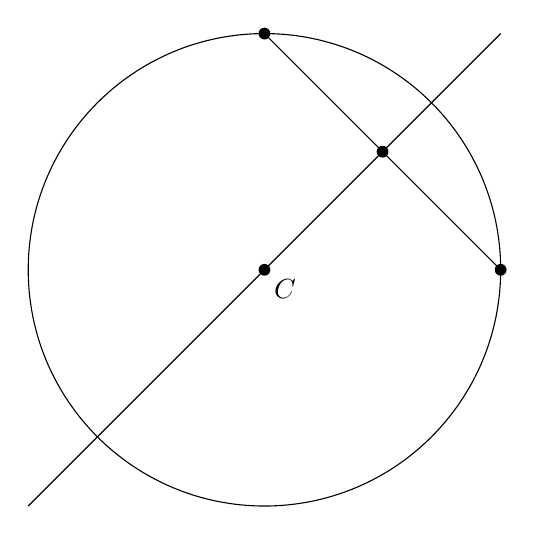
\begin{tikzpicture}
		\coordinate [label={below right:$C$}] (C) at (0, 0);
		\fill [black] (C) circle (0.075);
		\draw (C) circle [radius=3]; 
		\draw (-3,-3) -- (3,3);
		\fill [black] (1.5,1.5) circle (0.075);
		\fill [black] (0,3) circle (0.075);
		\fill [black] (3,0) circle (0.075);
		\draw (0,3) -- (3,0);

	\end{tikzpicture}

\end{center}

\section{asymptotes}
Asymptotes are imaginary lines that graphs will extend to but never touch. A good example of this is with the graph $y=x^{-1}$
which has two asymptotes. One on the x axis ($y = 0$) and one on the y axis ($x = 0$)

\begin{center}
	\begin{tikzpicture}
		\begin{axis}[
			xmin=-10, xmax=10,
    		ymin=-10, ymax=10,
			axis lines=middle
		]
			\addplot[samples=100,domain=-10:10] {x^(-1)};
		\end{axis}
	\end{tikzpicture}
\end{center}

\section{Exponentials and Logarythms}

\subsection{Laws of Logarythms}

\begin{gather}
	\log_{a}{x^y} = y\\
	\log_{a}{x} + \log_{a}{y} = \log_{a}{xy} \\
	\log_{a}{x} - \log_{a}{y} = \log_{a}{\frac{x}{y}} \\
	y\log_{a}{x} = \log_{a}{x^y}
\end{gather}

\subsubsection{Special Cases}

\begin{gather}
	\log_{a}{\frac{1}{x}} = \log_{a}{x^{-1}} = -\log_{a}{x} \\
	\log_{a}{a} = 1 \left \{a > 0, a \ne 1 \right \}\\
	\log_{a}{1} = 0 \left \{a > 0, a \ne 1 \right \}\\
\end{gather}

\subsection{Natural log}

\begin{gather}
	\ln{x} = \log_e{x}
\end{gather}

\subsection{Graphs}

Both $ln x$ and $e^x$ have one asymptote. In the case of $ln x$ it is the y axis ($x = 0$) and for $e^x$ it is the x axis ($y = 0$).
They are symetrical along the line $y=x$. The graphs have been plotted below:

\begin{center}
	\begin{tikzpicture}
		\begin{axis}[
			xmin=-10, xmax=10,
    		ymin=-10, ymax=10,
			axis lines=middle,
			tick style={draw=none},
			xticklabels={,,},
			yticklabels={,,}
		]
			\addplot[samples=100, domain=-10:3] {exp(x))};
			\addplot[samples=100, domain=0:10] {ln(x))};
			\addplot[dashed] {x};
		\end{axis}
	\end{tikzpicture}
\end{center}

\section{Tangents and Normals}
Normals are lines perpendicular to a surface where as tangents are lines
that touch the surface at a single point with the same gradient.

\begin{center}
	\begin{tikzpicture}
		\begin{axis}[
			xmin=-10, xmax=10,
    		ymin=-10, ymax=10,
			axis lines=middle
		]
			\addplot[samples=100,domain=-10:10] {x^2};
			\addplot[samples=100,domain=-10:10] {2 * 1 * x - 1^2};
			\addplot[samples=100,domain=-10:10] {1 - ((x - 1) / (2 * 1))};
		\end{axis}
	\end{tikzpicture}
\end{center}
The gradients of the tangents and normals have the following relationship
\begin{equation}
	m_n = - m_t^{-1}
\end{equation}
\\
Arbitrary tangent and normal functions ($f_t(x, a)$ and $f_n(x, a)$) of a given function $f(x)$ at a given offset $a$ can be given as follows:

\begin{gather}
	f_t(x, a) = f'(x)(x-a) + a^2 \\
	f_n(x, a) = a^2 -f'(x)^{-1}(x-a) \\
\end{gather}

\section{Factor theorem}
When given a polynomial $f(x) = ax^n + bx^{n-1} + \cdots + z $
An expression $(x + a)$ is a factor of $f(x)$ if $f(-a) = 0$.
\\
We can use this to rule to factorise higher order polynomials such as the following:

\begin{gather}
	f(x) = x^3 + 3x^2 + 3x + 1 \\
	f(-1) = (-1)^3 + 3(-1)^2 + 3(-1) + 1 = 0\\
	\therefore (x + 1) \text{ is a factor} \\
	f(x) = (x+1)b = x^3 + 3x^2 + 3x + 1
\end{gather}

\begin{center}
	\begin{tabular}{ c | c | c | c }
		$\times$ & $x^2$ & $2x$ & $1$\\ \hline
		$x$ & $x^3$ & $2x^2$ & $x$  \\ \hline
		$1$ & $x^2$ & $2x$ & $1$\\
	\end{tabular}
\end{center}

\begin{gather}
	f(x) = (x+1)(x^2 + 2x + 1) \\
	f(x) = (x+1)(x+1)(x+1) = (x+1)^3
\end{gather}

\enddocument
